%% Ultrainfinitism II
%%
%% Render with:
%%   lualatex ultrainfinitism-ii.tex && lualatex ultrainfinitism-ii.tex
%% (self-contained bibliography; no bibtex pass required)

\documentclass[]{article}
\usepackage{url}
\usepackage[hyperindex,breaklinks]{hyperref}
\IfFileExists{breakurl.sty}{\usepackage{breakurl}}{}
\usepackage{listings}
\lstset{basicstyle=\ttfamily\footnotesize,breaklines=true,frame=single,
        xleftmargin=1em,xrightmargin=0.5em}
\usepackage{float}
\restylefloat{table}
\usepackage{longtable}
\usepackage{booktabs}
\usepackage{array}
\usepackage{graphicx}
\usepackage[font=small,labelfont=bf]{caption}
\usepackage[skip=0pt]{subcaption}
\usepackage{amsfonts}
\usepackage{amsmath}
\usepackage{amssymb}
\usepackage{amsthm}
\usepackage{mathtools}
\usepackage{unicode-math}
\IfFileExists{newunicodechar.sty}{
  \usepackage{newunicodechar}
  \newunicodechar{∘}{\ensuremath{\circ}}
}{}
\IfFontExistsTF{Stix Two Math}{\setmathfont{Stix Two Math}}{\setmathfont{STIX Math}}

% Compatibility fallback for older TeX bundles.
\makeatletter
\providecommand{\headerps@out}{}
\makeatother

\usepackage{tikz}
\usetikzlibrary{arrows.meta,positioning,calc,decorations.pathreplacing,fit,backgrounds}

\newtheorem{theorem}{Theorem}
\newtheorem{lemma}[theorem]{Lemma}
\newtheorem{proposition}[theorem]{Proposition}
\newtheorem{corollary}[theorem]{Corollary}
\newtheorem{bridge}[theorem]{Bridge}
\theoremstyle{definition}
\newtheorem{definition}[theorem]{Definition}
\newtheorem{principle}[theorem]{Principle}
\theoremstyle{remark}
\newtheorem{remark}[theorem]{Remark}
\newtheorem{reading}[theorem]{Reading}

% \code as in the first essay, with line breaks allowed after underscores and dots of long names.
\newcommand{\codeus}{\textunderscore\allowbreak}
\newcommand{\code}[1]{\texttt{\let\_\codeus #1}}
\newcommand{\lpath}[1]{{\ttfamily\nolinkurl{#1}}}
\newcommand{\ty}[1]{\ensuremath{\mathtt{#1}}}
\newcommand{\Uf}{\mathcal{U}}
\newcommand{\limstar}{\ensuremath{M^{\!*}}}
\newcommand{\R}{\mathbb{R}}
\newcommand{\N}{\mathbb{N}}
\DeclareMathOperator{\uprod}{\textstyle\prod}
% New in the sequel.
\newcommand{\Om}{\Omega}
\newcommand{\Nstar}{\N^{*}}
\newcommand{\Pfin}{\mathcal{P}(\N)/\mathrm{fin}}
\newcommand{\meta}[1]{\lpath{Metaphysics/#1.lean}}
\newcommand{\step}[1]{\lpath{Step/#1.lean}}
\newcolumntype{L}[1]{>{\raggedright\arraybackslash}p{#1}}

\emergencystretch=8em
% Theorem headings carry long declaration names and module paths.
\tolerance=2000
\hbadness=3000

\title{Ultrainfinitism II:\\
       Infinite Wholes and the Boundary of Effing\\[4pt]
       {\large Sinkless collapse, labelled plurality, pointless algebras,\\
        bridges, two ineffabilities, and transforms of the transfinite}}
\author{Mettapedia Working Notes}
\date{\today}

\begin{document}
\maketitle

\begin{abstract}
The first essay read the finite as a principal-ultrafilter shadow of an infinite One and
anchored the reading in {\L}o\'s's theorem, credal envelopes and Stone duality. This sequel
sharpens the principle and tests it against new machine-checked results. \emph{Infinite wholes
are primary; finite information appears only as observation of them}---a prefix read below a
depth, an outcome under a budget, a coordinate, a clopen---\emph{never as their parts}. Four
results carry the sharpened principle. With no empties anywhere, extensional structure yields
exactly one thing, Aczel's $\Om=\{\Om\}$. Plurality needs labels: two labels already give
uncountably many leafless wholes, only countably many of which have a finite presentation, and no
bounded observation tells them all apart. A single whole can carry uncountably many
self-identifications. A complete atomless algebra has no points at all, so individuals appear only
when observation is cut down to finite joins and a free choice is made. Models assembled from
finite pieces---the cofinite core of the free ultrafilters, $\Pfin$, hyperfinite runs---are
treated explicitly as \emph{bridges}, not foundations. We then separate three senses of ``without
normal forms'', order what can be \emph{effed} (finitely and checkably presented) in a hierarchy
tied to the outcomes of bounded search, and distinguish two ineffabilities: one from symmetry (no
deterministic equivariant choice among indiscernibles) and one from self-reference (Lawvere's fixed-point
theorem). Transforms of infinite trees and runs converge, conserve their charges, fold silently and
pump without bound, each under stated hypotheses. The diagonal and symmetry theorems are finite,
checked statements; they eff exactly where effing must stop. Every result stated as proved names
its Lean declaration; readings and bridges are labelled as such.
\end{abstract}

\tableofcontents

%% ===================================================================
\section{Introduction}
\label{sec:intro}

The first essay \cite{UI1} argued that only the infinite is truly real and that every finite
object is a \emph{simulation}: the One read at a single coordinate by a principal ultrafilter. Its
Law of Oneish said that beneath the carvings there is one thing, and that carvings are how a
perspective makes a finite world to live in. Two bridge principles graded the step from
phenomenology to ontology: \emph{No-Atom} (if no boundary is absolute, there is no minimal, fully
separated individual) and \emph{Priority of the Whole} (a carving presupposes the manifold it
carves, not conversely). The mathematical home was the ultraproduct $\bigl(\uprod_i M_i\bigr)/\Uf$
with {\L}o\'s's theorem as the law of transfer, indexed explicitly as a relative One
$\mathrm{One}_{(M,\Uf)}$; the native home was atomless (gunky) mereology, welded by Stone duality to
perfect point-spaces in which no finitary point stands alone. Its ``Honest scope'' remark kept proved
results apart from the envisioned, and its Lean appendix transcribed the anchors.

\paragraph{The sharpened principle.} The first essay still let the finite appear as a coordinate
\emph{of} a product---one factor among the $M_i$. Read strictly, that concedes too much: a product is
assembled from its factors. The sequel takes the opposite order of construction as primary.

\begin{principle}[wholes first]
\label{prin:wholes}
Infinite wholes are primary. Finite information appears only as \emph{observation} of a whole: a
prefix (agreement below a depth), a budget (the outcome of a search cut off at depth $n$), a
coordinate (a principal ultrafilter), a clopen (a finite join of basic observations). It never
appears as a \emph{part} from which the whole is assembled.
\end{principle}

The difference is the difference between an initial algebra, whose elements are built from finite
parts, and a final coalgebra, whose elements are known by their finite observations
\cite{Rutten2000}. A model assembled from finite pieces can still be useful, and several are used
below. The algebra $\Pfin$, for instance, is atomless and has a perfect Stone space, and so is a
faithful image of the thesis; but its zero \emph{is} the class of all finite sets. Such a model is a
\emph{bridge}: it transports truth between finite observations and wholes, but it is not the
foundation, because it is made out of what the foundation is supposed to make.

\paragraph{Effing.} We say that a thing is \emph{effed} when a finite, checkable presentation
determines it: a finished certificate, a finite graph, a program, an approximation scheme with a
named limit. The ineffable is what no such presentation reaches. The paper's second half orders the
grades of effability and shows that the places where effing fails are themselves sharply effable.

\paragraph{What is new.}
\begin{enumerate}
\item \emph{The One by structure} (Section~\ref{sec:one}): sinkless collapse to $\Om$
  (Theorem~\ref{thm:sinkless}); plurality only through labels, uncountable and mostly without
  finite presentation (Theorem~\ref{thm:leafless}); one whole with uncountably many
  self-identifications (Theorem~\ref{thm:inner}); a complete atomless algebra with no points
  (Theorem~\ref{thm:pointless}); opaque atoms, the ``empty'' as a whole seen from outside
  (Theorem~\ref{thm:opaque}); and finite talk as distinction, which induces finite quotients of a
  whole rather than finite parts (Section~\ref{sec:shadow}).
\item \emph{Bridges} (Section~\ref{sec:bridges}): what every free One affirms is exactly what
  holds cofinitely (Bridge~\ref{thm:cofinite}); no ultrafilter is fixed by every symmetry, in one
  form shared with an observer theorem (Bridge~\ref{thm:symmetry}); and $\Pfin$
  (Bridge~\ref{thm:pfin}).
\item \emph{Three senses of ``without normal forms''} (Section~\ref{sec:normal}), including
  Lawvere's theorem for types and the collapse of every arrow model of rational types
  (Theorems~\ref{thm:lawvere}--\ref{thm:rationaltypes}).
\item \emph{A hierarchy of effability} tied to the outcomes of bounded search
  (Section~\ref{sec:hierarchy}, Theorem~\ref{thm:search}).
\item \emph{Two ineffabilities} (Section~\ref{sec:ineffable}): symmetric and diagonal.
\item \emph{Transforms over transfinite entities} (Section~\ref{sec:transforms}): $\omega$-limits
  (Theorem~\ref{thm:limits}), hyperfinite runs (Bridge~\ref{thm:hyperrun}), the quiet fold
  (Theorem~\ref{thm:quiet}) and the affine pump (Theorem~\ref{thm:pump}).
\end{enumerate}

\paragraph{Conventions.} A result is stated as a \emph{theorem} only when a named Lean~4
declaration proves it without \code{sorry}; the theorem heading names the declaration and its
module. Results numbered as a \emph{Bridge} are proved in the same sense. Module paths are
repository-relative; we abbreviate
\lpath{Mettapedia/Logic/Metaphysics/X.lean} as \meta{X} and
\lpath{Mettapedia/Languages/ProcessCalculi/ConstraintMultisetRewriting/Step/X.lean} as \step{X}.
Unless stated otherwise the anchors depend on at most the standard axioms \code{propext},
\code{Classical.choice} and \code{Quot.sound}; where a result uses less, we say so. A
\emph{bridge} is a model built from finite pieces and used to transfer truth. A \emph{reading} is an
interpretation of a theorem, offered as interpretation; nothing in a reading is claimed as proved.

%% ===================================================================
\section{The One by structure; plurality by carving}
\label{sec:one}

\subsection{Sinkless collapse: no empties, one thing}
\label{sec:sinkless}

Work with hypersets: sets under Aczel's anti-foundation axiom, in which every graph has exactly one
decoration and equality is bisimilarity \cite{AczelAFA, BarwiseMoss1996}. In the development the
axiom is a theorem about a model of hypersets, and $\Om=\{\Om\}$ is the hyperset pictured by a
one-node loop. Call a hyperset $x$ \emph{hereditarily nonempty} when every member of its transitive
closure, $x$ itself included, has a member.

\begin{theorem}[sinkless collapse; \code{hereditarilyNonempty\_iff\_eq\_quineAtom},
\code{eq\_of\_hereditarilyNonempty}, \code{decorate\_eq\_quineAtom\_iff\_sinkless}, \meta{UltrainfiniteSinkless}]
\label{thm:sinkless}
\leavevmode
\begin{enumerate}
\item A hyperset is hereditarily nonempty if and only if it is $\Om$. In particular any two
  hereditarily nonempty hypersets are equal.
\item A graph pictures $\Om$ at a node exactly when no sink (node without children) is reachable
  from that node.
\item \emph{Control} (\code{sink\_plurality}): with a sink, plurality appears: $\emptyset\neq\{\emptyset\}$,
  and neither is hereditarily nonempty.
\end{enumerate}
The proof exhibits ``both are hereditarily nonempty'' as a bisimulation of the membership graph
(\code{isBisimulation\_hereditarilyNonempty}) and applies strong extensionality. Parts~1--2 use no
choice.
\end{theorem}

The collapse is a consequence of \emph{extensional bisimulation}: hypersets with bisimilar membership
graphs are equal. It owes nothing to any principle about identity proofs. Nor is the surviving whole
empty: $\Om$ has a member, namely itself, and every member of its closure is $\Om$
(\code{eq\_quineAtom\_of\_inClosure}).

Every sinkless presentation pictures the same whole, whatever its shape: the loop, the two-cycle,
and the full binary tree below are three pictures of one thing (Figure~\ref{fig:sinkless}).

\begin{figure}[H]
\centering
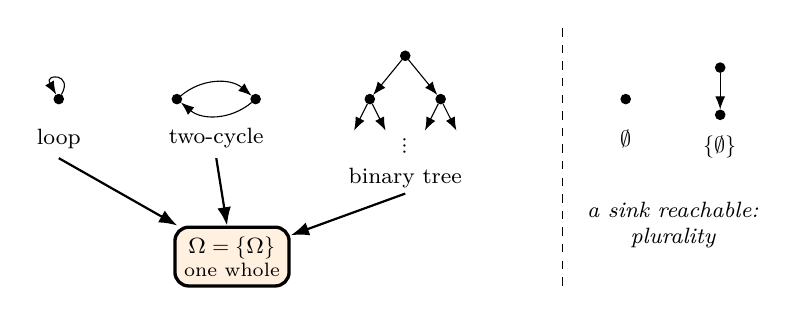
\begin{tikzpicture}[>=Latex, every node/.style={font=\footnotesize},
  nd/.style={circle, draw, fill=black, inner sep=1.2pt}]
  % loop
  \node[nd] (l) at (0,0) {};
  \draw[->] (l) to[out=60,in=120,looseness=12] (l);
  \node at (0,-0.5) {loop};
  % two-cycle
  \node[nd] (a) at (1.5,0) {};
  \node[nd] (b) at (2.5,0) {};
  \draw[->] (a) to[bend left=40] (b);
  \draw[->] (b) to[bend left=40] (a);
  \node at (2,-0.5) {two-cycle};
  % binary tree
  \node[nd] (r) at (4.4,0.55) {};
  \node[nd] (r0) at (3.95,0) {};
  \node[nd] (r1) at (4.85,0) {};
  \draw[->] (r)--(r0); \draw[->] (r)--(r1);
  \draw[->] (r0)--(3.75,-0.4); \draw[->] (r0)--(4.15,-0.4);
  \draw[->] (r1)--(4.65,-0.4); \draw[->] (r1)--(5.05,-0.4);
  \node at (4.4,-0.6) {$\vdots$};
  \node at (4.4,-1.0) {binary tree};
  % brace to Omega
  \node[draw, very thick, rounded corners=5pt, fill=orange!12, align=center]
    (om) at (2.2,-2.0) {$\Om=\{\Om\}$\\[-1pt]{\scriptsize one whole}};
  \draw[->, thick] (0,-0.75) -- (om);
  \draw[->, thick] (2,-0.75) -- (om);
  \draw[->, thick] (4.4,-1.2) -- (om);
  % sinks
  \node[nd] (s0) at (7.2,0) {};
  \node at (7.2,-0.5) {$\emptyset$};
  \node[nd] (s1) at (8.4,0.4) {};
  \node[nd] (s2) at (8.4,-0.2) {};
  \draw[->] (s1)--(s2);
  \node at (8.4,-0.6) {$\{\emptyset\}$};
  \node[align=center, font=\footnotesize\itshape] at (7.8,-1.6)
     {a sink reachable:\\ plurality};
  \draw[dashed] (6.4,0.9) -- (6.4,-2.4);
\end{tikzpicture}
\caption{Sinkless collapse (Theorem~\ref{thm:sinkless}). Every sinkless graph pictures $\Om$ at
every node; plurality of pure sets begins only where a sink---an empty---is reachable.}
\label{fig:sinkless}
\end{figure}

\begin{reading}[the Law of Oneish, by structure]
\label{read:oneish}
In well-founded set theory every set reaches $\emptyset$, so the empty set is where all
distinctions among pure sets bottom out. Theorem~\ref{thm:sinkless} supplies the complement: once no
empty is reachable anywhere, extensional structure has exactly one thing to say. Pure plurality is
\emph{sourced} in emptiness. An ultrainfinitist who denies finite atoms and empty individuals
therefore cannot get plurality from pure membership at all; it must come from somewhere else. The
next subsection shows where.
\end{reading}

\subsection{Distinctions need labels: leafless wholes}
\label{sec:leafless}

Read a tree by its labels at paths, as a function from finite lists of child indices to labels. A
tree is \emph{leafless} when it is well formed and every label present in it has a child; so it has
no variable or constant leaves and is built from function symbols of positive arity alone.

\begin{theorem}[plurality by labels; \meta{UltrainfiniteLeafless}]
\label{thm:leafless}
Let $\sigma$ be a signature.
\begin{enumerate}
\item \emph{No leafless tree is finite} (\code{Leafless.infinite\_support},
  \code{Leafless.infinite\_support\_sub}, \code{not\_leafless\_ofTerm}): it is present at infinitely
  many paths, so is every subtree, and no finite term reads as one.
\item \emph{Two symbols give uncountably many} (\code{not\_countable\_setOf\_leafless}): if $f\neq g$
  have positive arity, the leafless trees are uncountable.
\item \emph{Few have a finite presentation} (\code{countable\_leafless\_rational},
  \code{exists\_leafless\_not\_rational}): over countably many symbols the rational leafless trees
  (finitely many distinct subtrees) are countable, each the unfolding of a finite code; hence some
  leafless tree is not rational.
\item \emph{No bounded observation decides identity} (\code{exists\_ne\_agree\_below}): for every depth
  $d$ there are two distinct leafless trees with the same label at every path shorter than $d$.
\item \emph{Control: one symbol, one whole} (\code{existsUnique\_leafless\_of\_subsingleton}): with at
  most one function symbol, and that of positive arity, there is exactly one leafless tree.
\end{enumerate}
\end{theorem}

The hypothesis of part~2, two distinct symbols of positive arity, is minimal, as part~5 shows.
With one unary symbol the only leafless tree is $f(f(f(\cdots)))$, whose membership reading is again
$\Om$. So Theorems~\ref{thm:sinkless} and~\ref{thm:leafless} together locate plurality exactly:
without sinks and without a second label, there is one whole; a second label, and no leaf at all,
already gives a continuum of wholes.

\begin{reading}[plurality by carving]
\label{read:carving}
Labels are the first carving. The wholes they distinguish are not assembled from labelled finite
pieces: parts~1 and~4 say there are no finite pieces to assemble from, and no finite inspection
closes the question of which whole is in view. Part~3 says that most of these wholes cannot be
named by a finite graph at all. Plurality is real, but it is plurality of infinite wholes, carved
by labels and observed by prefixes.
\end{reading}

\subsection{One whole with inner diversity}
\label{sec:inner}

The full binary tree has the finite Boolean lists as nodes and an edge from $p$ to $p\mathbin{+\!\!+}[b]$.
Each subtree below the root is again the full binary tree (\code{child\_cons\_iff}), so as an iterated
multiset it is $T=\{T,T\}$. It is sinkless.

\begin{theorem}[one with inner diversity; \code{inner\_diversity}, \meta{UltrainfiniteInnerDiversity}]
\label{thm:inner}
\leavevmode
\begin{enumerate}
\item The edge-preserving permutations of the nodes form a subgroup \code{treeAut}, and it is
  uncountable (\code{not\_countable\_treeAut}): choosing at each node whether to swap its children
  is an automorphism (\code{swapPerm\_mem\_treeAut}), and distinct choices give distinct automorphisms
  (\code{swapPerm\_injective}).
\item \emph{Control: as a set it is one thing.} The tree pictures $\Om$ at every node
  (\code{decorate\_binaryTree}), and every automorphism of the membership structure of hypersets is
  the identity (\code{eq\_self\_of\_mem\_automorphism}).
\end{enumerate}
\end{theorem}

\begin{reading}[connected, not contractible]
\label{read:connected}
As an object, $T$ is one: read extensionally it is $\Om$, and $\Om$ has exactly one
self-identification. As a \emph{structure}, $T$ has uncountably many. In the vocabulary of homotopy
type theory \cite{HoTTBook} this is the profile of a type that is connected (there is one object
up to identification) but not contractible (its self-identifications do not all coincide). The
groupoid model of Hofmann and Streicher is the classical place where identity carries such content
\cite{HofmannStreicher1998}. We offer this only as a reading of one object with an uncountable
automorphism structure, and the reading rests on Theorem~\ref{thm:inner}, not on any choice of
identity principle. In particular it is not a consequence of dropping Streicher's axiom~K: failure of
uniqueness of identity proofs does not by itself give connectedness, nontrivial loops, or the
equality of all objects, which are separate properties. Lean's equality is proof-irrelevant and
validates~K, so it cannot itself carry a nontrivial group of self-identifications; the development
therefore carries identity as explicit structure, the subgroup \code{treeAut}, rather than as
equality. The theorem is about that structure; the homotopical vocabulary is interpretation.
\end{reading}

\subsection{Stone points against locale points}
\label{sec:pointless}

The first essay proved that a Boolean algebra is atomless exactly when its Stone space is perfect
(\code{isGunky\_iff\_perfect\_stoneSpace}, \lpath{Mettapedia/Logic/StoneGunkDuality.lean}). A perfect Stone
space still has points: ultrafilters exist in every nontrivial Boolean algebra by the Boolean prime
ideal theorem \cite{Stone1936, Johnstone1982}, a form of choice. Ultrafilters respect only
\emph{finite} joins. Ask instead for the points of the algebra as a locale---completely prime filters,
which respect \emph{all} joins---and the answer changes.

\begin{theorem}[a complete atomless algebra has no points; \code{exists\_atom\_of\_point},
\code{isEmpty\_point\_of\_isGunky}, \code{isEmpty\_point\_regular\_opens},
\lpath{Mettapedia/SetTheory/CarveOuts/HeytingValued/Gunky.lean}]
\label{thm:pointless}
\leavevmode
\begin{enumerate}
\item In a complete Boolean algebra every point (completely prime filter) is generated by an atom.
  Hence a complete atomless Boolean algebra has no point at all.
\item For a Hausdorff space with no isolated point, the regular open sets form an atomless complete
  Boolean algebra with no point. The frame of all open sets of a $T_1$ space with no isolated point
  is atomless, has a point for every point of the space, and none of its points is principal
  (\code{not\_isPrincipal\_opens}).
\item Cantor space and the real line are witnesses (\code{cantorGunkyWitness},
  \code{realGunkyWitness}).
\end{enumerate}
\end{theorem}

The three cases line up as follows.

\begin{table}[H]
\centering\small
\begin{tabular}{@{}L{0.18\textwidth}cL{0.12\textwidth}L{0.25\textwidth}L{0.17\textwidth}@{}}
\toprule
Algebra & complete? & atoms & Stone points (ultrafilters) & locale points \\
\midrule
$\mathcal{P}(\N)$ & yes & singletons & the coordinates, isolated; free ones by choice & the
  coordinates only \\
$\Pfin$ & no & none & by choice only; none isolated & --- (not a frame) \\
regular opens of $2^{\N}$ & yes & none & by choice only; none isolated & none at all \\
\bottomrule
\end{tabular}
\caption{Points, three ways. Atoms of $\mathcal{P}(\N)$ are the singletons (the first essay's
\code{isAtom\_set\_singleton}, \code{not\_isGunky\_set}); its locale points sit at atoms by
Theorem~\ref{thm:pointless}, part~1. The second row is Bridge~\ref{thm:pfin}. In the third row the
locale points are Theorem~\ref{thm:pointless}, part~2, and ``none isolated'' is the first essay's
duality applied to an atomless algebra.}
\label{tab:points}
\end{table}

\begin{reading}[the pointless One]
\label{read:pointless}
The complete atomless One has no individuals at all. Individuals appear only when observation is
cut down to finite joins (passing from a locale to a Boolean algebra of clopens) \emph{and} a free
choice is made (an ultrafilter). This is the home Johnstone argued for in ``the point of pointless
topology'' \cite{Johnstone1983}, here doing ultrainfinitist work: a point is an act of observation
with a choice in it, not a constituent of the space.
\end{reading}

\subsection{Opaque atoms: an empty is a whole seen from outside}
\label{sec:opaque}

The first essay's objection section asked what becomes of the empty set and the urelement in an
infinite-native foundation. A many-coloured construction of set universes gives one answer. Each
colour builds sets of its own objects, and every colour it sees contributes its objects as
\emph{opaque atoms}: references that keep their identity but expose no membership.

\begin{theorem}[reference without containment; \code{atom\_memberless}, \code{atom\_injective},
\code{atomEmbedding}, \code{transparent\_reflection\_impossible},
\lpath{Mettapedia/SetTheory/ColoredOpaqueUniverses.lean}]
\label{thm:opaque}
An atom of colour $c$ whose payload is an object of colour $d$ has no members of colour $c$,
whatever the payload holds; yet distinct payloads give distinct atoms, so the whole universe of $d$
embeds into that of $c$ as atoms. A \emph{transparent} reflection---an injective encoding of a
universe's own powerclass into itself---is impossible (Cantor).
\end{theorem}

\begin{reading}[the empty as an outside view]
\label{read:opaque}
From inside colour $c$, an atom looks exactly like an empty: it has no members. From colour $d$ it
is a whole object with all its structure. ``Empty'' is thus a property of the \emph{view}, not of
the thing. Opacity is what separates mutual reflection from unrestricted comprehension: the veil
lets every universe contain every other as references, while Cantor's diagonal forbids any
universe to contain itself transparently. The construction is stated at a finitary,
well-founded syntactic tier; its coalgebraic, non-well-founded version is not claimed here.
\end{reading}

\subsection{Finite talk as distinction, in the shadow of the infinite}
\label{sec:shadow}

What, then, does finite talk about a whole do, if it never names a finite part? It draws
distinctions. A yes/no observation is an element $b$ of a Boolean algebra $B$ of observations:
``inside $b$'' or ``inside its complement''. Finitely many observations $b_1,\dots,b_n$ generate a
finite subalgebra $B_0\subseteq B$. Every finite Boolean algebra is atomic and isomorphic to the
powerset of its atoms; the atoms of $B_0$ are the nonzero meets $\pm b_1\wedge\dots\wedge\pm b_n$, there
are at most $2^n$ of them, and they partition the top \cite{GivantHalmos2009}. Dually, $B_0$ is a
partition of the Stone space $S(B)$ into finitely many clopens, that is, a continuous surjection of
$S(B)$ onto a finite discrete space; and $S(B)$ is the inverse limit of these finite quotients over
the finite subalgebras of $B$ \cite{Johnstone1982}.

When $B$ is gunky, these atoms belong to the shadow, not to the whole. $B$ has no atoms at all, and
its Stone space has no isolated point (\code{isGunky\_iff\_perfect\_stoneSpace}); so each atom of
$B_0$ splits again in $B$, and each cell of the finite partition contains infinitely many points.
Finitely many distinctions never pick out a finite \emph{part} of a whole; they induce a finite
\emph{quotient} of it, a shadow.

\begin{theorem}[finite shadows; \meta{UltrainfiniteShadows}, \meta{UltrainfiniteShadowsStone},
\meta{UltrainfiniteShadowsCantor}]
\label{thm:shadows}
\leavevmode
\begin{enumerate}
\item Finitely many distinctions generate a finite subalgebra (\code{finite\_closure}) whose atoms,
  the \emph{shadow atoms}, partition the top (\code{isLUB\_shadowAtoms}); the whole is the directed
  union of its finite shadows (\code{iUnion\_shadows\_eq\_univ}).
\item An algebra is gunky exactly when no shadow atom of any finite shadow is an atom of the whole
  (\code{isGunky\_iff\_forall\_shadowAtoms\_not\_isAtom}); in a gunky algebra every shadow atom splits
  in a finer shadow (\code{exists\_finer\_shadow\_split}); a finest shadow exists exactly when the
  algebra is finite (\code{finite\_iff\_exists\_shadow\_forall\_isAtom}).
\item Dually, a finite shadow is a finite clopen quotient of the Stone space; a shadow atom is an atom
  of the whole exactly when its class is a single point (\code{isAtom\_iff\_fibre\_eq\_singleton}), and
  in a gunky algebra every class is infinite (\code{shadowMap\_fibre\_infinite}).
\item For Cantor space, the space is the inverse limit of its depth-$n$ shadows
  (\code{shadowLimitHomeomorph}, with the universal property \code{existsUnique\_lift}); each class is
  homeomorphic to the whole (\code{fibreHomeomorph}); and finitely many clopen distinctions never
  single out a point (\code{exists\_ne\_of\_finite\_distinctions}).
\end{enumerate}
\end{theorem}

\noindent The inverse-limit presentation of a general Stone space by its finite shadows is not yet
formalized (Section~\ref{sec:scope}).

\paragraph{Tolerances as observers.} The distinction calculus, already formalized in the development,
reads an observer the same way, with grades \cite{GoertzelHyperseed}. A \emph{tolerance} is a bounded,
reflexive, symmetric similarity on states, not assumed transitive; its complementary distance may be
zero on distinct states. For a tolerance satisfying the triangle law, zero distance is an
equivalence, and the observer it induces is the quotient map: two states look the same to it exactly
when the tolerance cannot tell them apart (\code{quotientObserver\_equal\_iff},
\lpath{Mettapedia/Cybernetics/DistinctionCalculus/Observation.lean}). A finite report induces the
crisp case: indistinguishable exactly when the reports agree (\code{ofReport\_indistinguishable},
\lpath{Mettapedia/Cybernetics/DistinctionCalculus/Basic.lean}). In both cases the observer's world is a
quotient of the states, never a part of them.

\paragraph{Computation in the same picture.} A computable function on infinite objects---streams,
Cantor space, infinite trees---is continuous: each output distinction depends on finitely many input
distinctions \cite{Weihrauch2000}. On Cantor space the finite-interaction form is formalized: a map
into a discrete space is continuous exactly when it depends only on a fixed finite prefix, and
exactly when a finite decision tree computes it (\code{continuous\_iff\_exists\_depth},
\code{continuous\_iff\_exists\_decisionTree}, \meta{UltrainfiniteShadowsCantor}); a uniform
oracle notion of computability is not formalized. An observer of the distinction calculus that
resolves only to depth $n$ has at most $2^n$ classes, all infinite (\code{ResolvesWithin.finite\_quotient},
\code{ResolvesWithin.infinite\_class}, \meta{UltrainfiniteShadowsDistinction}). The productive
transforms of Section~\ref{sec:limits} are an
instance by definition: an output label below depth $d+1$ depends only on input labels below depth
$d$ (\code{Productive}, \step{TransfiniteLimits}).

\begin{reading}[the computable as a shadow]
\label{read:shadow}
The computable is the shadow that finite interactions with infinite wholes leave behind. A program
consults finitely many distinctions of its input before committing to each distinction of its
output, so what it computes factors, at every stage, through a finite quotient of the input. The
``computable'' rung of the effability hierarchy (Section~\ref{sec:hierarchy}) is in this sense the
rung of continuous shadows.
\end{reading}

%% ===================================================================
\section{Bridges: the indexed One}
\label{sec:bridges}

The results of this section are \emph{bridges}. Each concerns models defined by finiteness over
coordinates---cofinite sets, sets modulo finite differences, ultrapowers of families---and the free
ultrafilters they mention exist only by choice. They transport truth between observation and
whole; they do not ground the whole.

\subsection{B1: the cofinite core and {\L}o\'s}
\label{sec:cofinite}

Call an ultrafilter \emph{free} (\code{IsFree}) when it is the principal ultrafilter of no point.
For ultrafilters this is the same as refining the cofinite filter (\code{isFree\_iff\_le\_cofinite})
and the same as containing no finite set (\code{isFree\_iff\_finite\_notMem}); free ultrafilters exist
exactly on infinite index sets (\code{exists\_free\_iff\_infinite}). Write
$\mathrm{UltraTrue}(\Uf,P)$ for ``$P$ holds at $\Uf$-almost every coordinate'', the verdict of the
relative One of the first essay.

\begin{bridge}[the effable core of the free One; \meta{UltrainfiniteCofinite}, \meta{UltrainfiniteCofiniteLos}]
\label{thm:cofinite}
For every index set $I$ and every family $P:I\to\mathrm{Prop}$:
\begin{enumerate}
\item \emph{The cofinite filter is the meet of the free ultrafilters}
  (\code{mem\_cofinite\_iff\_forall\_free}, \code{iSup\_free\_eq\_cofinite}): a set is cofinite exactly
  when every free ultrafilter contains it.
\item \emph{What every free One affirms is what holds cofinitely}
  (\code{forall\_free\_ultraTrue\_iff}): $\bigl(\forall\Uf\text{ free},\ \mathrm{UltraTrue}(\Uf,P)\bigr)$
  iff $\{i:\neg P\,i\}$ is finite.
\item \emph{Some free One affirms what holds infinitely often}
  (\code{exists\_free\_ultraTrue\_iff}).
\item \emph{The free dial} (\code{freeOpen\_iff}): two free Ones disagree about $P$ exactly when $P$
  holds at infinitely many coordinates and fails at infinitely many.
\item \emph{{\L}o\'s forms} (\code{forall\_free\_uprod\_iff}, \code{exists\_free\_uprod\_iff},
  \code{freeOpen\_uprod\_iff}): for a family of first-order structures $A_i$ and a sentence $\varphi$,
  $\varphi$ holds in every free ultraproduct iff it holds at all but finitely many $A_i$; in some
  free ultraproduct iff at infinitely many; and the free ultraproducts disagree iff both sets are
  infinite.
\end{enumerate}
\emph{Controls on $\N$}: ``nonzero'' holds in every free One (\code{forall\_free\_ne\_zero}),
``zero'' in none (\code{not\_exists\_free\_eq\_zero}), and ``even'' is open among them
(\code{freeOpen\_even}).
\end{bridge}

Part~5 composes the wrapper form of {\L}o\'s's theorem of the first essay
(\code{ultraTrue\_iff\_uprod}, \meta{UltrainfinitismLosTransfer}) with parts~2--4.

\begin{reading}[effable and chosen]
\label{read:effable-core}
The cofinite filter is defined without choice; the free ultrafilters are not. Bridge~\ref{thm:cofinite}
says that the meet of all the choices is exactly the choice-free part. So the indexed One divides
cleanly: what holds \emph{eventually} can be effed, and is affirmed by every free perspective;
everything else depends on which free ultrafilter is taken, which is a choice. The first essay's
credal width measured disagreement among perspectives; here the free perspectives disagree exactly on
that remainder (part~4).
\end{reading}

\subsection{B2: no symmetric One}
\label{sec:symmetry}

\begin{bridge}[no symmetric choice of a free One; \meta{UltrainfiniteSymmetry}, \meta{UltrainfiniteSymmetryObserver}]
\label{thm:symmetry}
\leavevmode
\begin{enumerate}
\item \emph{The shared form} (\code{select\_ne\_of\_fixed}, no axioms): if a selection---a
  function, hence deterministic---commutes with a symmetry, then at a point the symmetry fixes, the
  selection is neither member of a pair the symmetry exchanges.
\item \emph{Ultrafilters} (\code{map\_ne\_of\_preimage\_eq\_compl}): a map that carries a set onto its
  complement moves every ultrafilter. In particular the swap of $2k$ and $2k+1$ moves every
  ultrafilter on $\N$ (\code{map\_evenOddSwap\_ne}), so \emph{no ultrafilter on $\N$ is fixed by every
  permutation} (\code{no\_permutation\_invariant\_ultrafilter}).
\item \emph{Control} (\code{map\_swap\_eq\_of\_isFree}, \code{hyperfilter\_swap\_control}): every free
  ultrafilter is fixed by every transposition, hence by every permutation that moves finitely many
  points.
\item \emph{The observer instance} (\code{no\_equivariant\_selection\_of\_shared}): an observer's
  deterministic selection that is equivariant under the stated renaming action, with no choice fixed
  in advance, selects neither member of a pair exchanged by an automorphism of its record. That this is literally the observer library's theorem
  \code{no\_equivariant\_selection} (\step{ObserverChoices}) is checked by \code{rfl}
  (\code{no\_equivariant\_selection\_of\_shared\_eq}).
\end{enumerate}
\end{bridge}

The two obstructions in part~2 and part~4 are instances of one form, and neither is an instance of
the other: the ultrafilter theorem concerns a selection every ultrafilter makes (``the half of
$\{S,S^{c}\}$ it contains''), so it concludes that no ultrafilter is fixed at all, while the observer
theorem concerns records and their renamings. What a free ultrafilter decides is invisible to finite
changes (part~3); only an infinite symmetry moves it. Beyond the formal statement, ZF without choice
does not prove that a free ultrafilter on $\N$ exists \cite{Feferman1965}: the free One is not
merely unsymmetric, it is unconstructed.

\subsection{\texorpdfstring{B3: $\Pfin$}{B3: P(N)/fin}}
\label{sec:pfin}

\begin{bridge}[$\Pfin$; \code{instBooleanAlgebraGerm}, \code{coe\_eq\_bot\_iff}, \code{isGunky\_setModFinite},
\code{perfectSpace\_stoneSpace\_setModFinite}, \meta{UltrainfiniteSetModFinite}]
\label{thm:pfin}
Germs along a filter of functions into a Boolean algebra form a Boolean algebra, computed pointwise.
For the cofinite filter on $\N$ and \code{Prop} this is $\Pfin$, the subsets of $\N$ with finite
differences ignored. Its zero is the class of all finite sets; it has no atoms, since every infinite
set splits into its members of even and of odd rank; and its Stone space is perfect.
\end{bridge}

\begin{remark}[why a bridge]
\label{rem:pfin-bridge}
$\Pfin$ is the clearest image of the thesis inside classical mathematics: infinitely many empties
(every finite set) identified into one zero, no atom, no isolated point. Classically its Stone space
is $\Nstar=\beta\N\setminus\N$, the space of free ultrafilters on $\N$
\cite{ComfortNegrepontis1974, vanMill1984}. But it is built from the subsets of $\N$, hence from the
finite, and its zero is defined as the finite sets. It is therefore a bridge in the sense of
Principle~\ref{prin:wholes}. The identification of its Stone points with the free ultrafilters is
classical and is not proved in the development (Section~\ref{sec:scope}).
\end{remark}

%% ===================================================================
\section{Three senses of ``without normal forms''}
\label{sec:normal}

Ultrainfinitist slogans often say that wholes ``have no normal form''. An objection stands against
the naive version, and it is worth stating first.

\paragraph{The objection.} In a final coalgebra, bisimilar behaviours are \emph{equal}
\cite{Rutten2000, AczelAFA}. So each stream in Cantor space, each hyperset, each rational tree is
already canonical as a denotation. The development agrees: rational trees are equal exactly when
their presenting graphs are bisimilar (\code{unfold\_eq\_iff}, \step{RationalTrees}); unification over
them is unitary, with a canonical solved form built from the classes of a closure
(\code{classTree}, \step{RationalUnification}) and computed as a finite graph (\code{solvedGraph},
\step{RationalSolvedForm}). ``No normal form'' cannot simply mean ``no canonical denotation''.

Three precise senses survive. They concern \emph{representatives}, not denotations.

\subsection{No finite, well-founded representative}
\label{sec:nf-finite}

The leafless wholes of Theorem~\ref{thm:leafless} have no finite term reading
(\code{not\_leafless\_ofTerm}); the rational tree $f(f(f(\cdots)))$ solving $X=f(X)$ has none either.
The candidate step of Section~\ref{sec:transforms} makes the contrast operational: the firing that
tells $X=f(X)$ is refused over finite trees at every configuration (\code{tellLoopFinite\_refused},
\step{RationalStep}), admitted over rational trees from no knowledge (\code{tellLoop\_admitted}), and
its run ends in knowledge solved by $X:=f(f(f(\cdots)))$ (\code{tellLoop\_run}). The $\omega$-limits of
Theorem~\ref{thm:limits} are of the same kind: each iterate is finite, the limit is not.

\subsection{No canonical representative without breaking a symmetry}
\label{sec:nf-symmetry}

Configurations that differ only by a private renaming of names form orbits. Picking one member per
orbit is a selection, and Bridge~\ref{thm:symmetry} limits selections: no deterministic selection
that commutes with renaming can pick a member of a pair that a symmetry exchanges. In the nominal
setting, where names carry no order, an invariant choice of orbit representative must be fixed by
every renaming, and in general there is none \cite{Pitts2013}. The development records the
alternative directly: every equivalence has a canonical form \emph{by choice}
(\code{Canonicalizer.choose}, \step{Fold}), and computing one is left to a profile. Canonical forms on
a computer exist because its names are ordered; ordering the names is a choice that fixes the gauge.
Even a minimal presentation of a rational tree is unique only up to renaming its nodes, so making it a
single datum asks again for an order on names.

\subsection{No normal form at self-containing types}
\label{sec:nf-types}

The third sense is the sharpest, and it is a theorem about logic rather than data. Lawvere's
fixed-point theorem \cite{Lawvere1969, Yanofsky2003} holds for types in the following form.

\begin{theorem}[Lawvere for types; \code{lawvere\_fixedPoint}, \code{diagonalFix\_spec}, \meta{UltrainfiniteLawvere}]
\label{thm:lawvere}
If $e:A\to(A\to B)$ is surjective, every $f:B\to B$ has a fixed point; with a section of $e$ the fixed
point is the term $e\,(s\,g)\,(s\,g)$ with $g=\lambda a.\,f(e\,a\,a)$, the shape of
$(\lambda x.\,f(xx))(\lambda x.\,f(xx))$. \code{lawvere\_fixedPoint} depends on no axioms. Corollaries:
\begin{enumerate}
\item \emph{Cantor} (\code{not\_surjective\_prop}, \code{cantor\_surjective}): negation has no fixed
  point in \code{Prop}, so no $A\to(A\to\mathrm{Prop})$ is surjective;
\item \emph{Curry} (\code{nonempty\_of\_surjective}): a codomain reached by a point-surjection is
  inhabited, and (\code{subsingleton\_of\_surjective}) has at most one element;
\item \emph{the self-containing type is a One} (\code{unique\_of\_equiv\_arrow}): a type
  $X\simeq(X\to X)$ has exactly one element; \code{PUnit} is such a type and \code{Bool} is not
  (\code{punitEquivArrow}, \code{not\_nonempty\_bool\_equiv\_arrow});
\item \emph{Tarski} (\code{no\_truth\_predicate}, no choice): there is no $\mathrm{Tr}:X\to\mathrm{Prop}$
  with a substitution through which every predicate on $X$ is defined by a code.
\end{enumerate}
\end{theorem}

\begin{theorem}[rational types collapse; \code{omega\_typable}, \code{omega\_no\_normal\_form},
\code{cyclic\_type\_breaks\_normalization}, \step{RationalTypeControl};
\code{rarrow\_curryType}, \code{ArrowModel.unique\_carrier}, \code{occurs\_check\_keeps\_models},
\meta{UltrainfiniteLawvereTypes}]
\label{thm:rationaltypes}
\leavevmode
\begin{enumerate}
\item Over finite types, self-application $\lambda x.\,xx$ is untypable
  (\code{selfApplication\_untypable}). Over rational types,
  $\Om=(\lambda x.\,xx)(\lambda x.\,xx)$ is typable at the rational type $T=T\to T$, and $\Om$ has no
  normal form: its only reduct is itself.
\item Every rational type $b$ has a Curry type $C$ with $C=C\to b$.
\item \emph{Every arrow model is trivial}: in every interpretation of the rational types as types
  that reads the arrow as the function type up to equivalence, every rational type---$T=T\to T$
  included---has exactly one element.
\item \emph{Control}: the finite types have an arrow model with a two-element base type
  (\code{FiniteArrowModel.bool\_nontrivial}).
\end{enumerate}
\end{theorem}

Here $T=T\to T$ is exactly Lawvere's hypothesis: $T$ maps onto $T^{T}$. So the non-normalizing
term and the collapse of models are two faces of one diagonal. This is why the rational-tree fibre of
the candidate step admits cyclic \emph{data} but keeps the occurs check for \emph{types}: a
self-containing type logic inhabits every type and collapses every model in types.
\emph{Data may lack normal forms; the logic that reads it cannot contain itself.}

The collapse in part~3 decides equality classically and is a fact about types read as sets of all
functions. In domain-theoretic models a nontrivial $D\cong[D\to D]$ exists, because the arrow there
denotes only the continuous functions \cite{Scott1972}. The theorem is therefore about the type
discipline that uses the full function space, which is the one a proof assistant's logic uses.

\subsection{The objection answered}
\label{sec:nf-answer}

The objection is right about denotations and is in fact the thesis. A final coalgebra makes the
\emph{whole} canonical: identity is behaviour, and behaviour is infinite. What is not canonical is
any finite \emph{presentation}: one rational tree has infinitely many presenting graphs, related by
bisimulation; one orbit has no invariant representative; and at a self-containing type the logic
that would read a normal form collapses. The three senses are three ways in which the finite fails to
be the measure of the whole, while the whole is perfectly determinate.

%% ===================================================================
\section{The hierarchy of effability}
\label{sec:hierarchy}

What can a finite presentation do? Table~\ref{tab:hierarchy} orders the grades. Each rung names the
certificate that effs an object at that rung, and, where the development has one, the anchor that
makes the certificate precise.

\begin{table}[H]
\centering\small
\begin{tabular}{@{}L{0.2\textwidth}L{0.3\textwidth}L{0.42\textwidth}@{}}
\toprule
Rung & Certificate & Anchor or source \\
\midrule
finished observation & a search that finished & status \code{finished}; \code{run\_eq\_of\_finished},
  \code{refuted\_sound} (\step{SearchSpace}) \\
rational & a finite graph & \code{IsRational}, \code{rational\_iff\_unfold}; equality decided to a
  bounded depth, \code{unfold\_eq\_iff\_agree} \\
computable & a program & Turing \cite{Turing1936} \\
left-c.e.\ & answers that only grow & \code{run\_mono}; Chaitin's $\Om$ \cite{Chaitin1975} \\
limit ($\Delta^0_2$) & conjectures that settle & the first essay's \S(A) \cite{UI1};
  Gold, Putnam, Shoenfield \cite{Gold1965, Putnam1965, Shoenfield1959} \\
definable & a name, not an approximation & e.g.\ the second jump $\emptyset''$ \\
arbitrary & none & ineffable relative to a fixed language \\
\bottomrule
\end{tabular}
\caption{The hierarchy of effability: finished $<$ rational $<$ computable $<$ left-c.e.\ $<$ limit
$<$ definable $<$ arbitrary. Each inclusion is strict; the witnesses are standard (an infinite
rational tree; a computable non-periodic stream; $\Om$; $1-\Om$; $\emptyset''$; a counting argument).}
\label{tab:hierarchy}
\end{table}

\subsection{The rungs and the outcomes of search}
\label{sec:hier-search}

The lower rungs are tied to an algebra of bounded-search outcomes. An outcome is a multiset of
answers with a status, \emph{finished} (the search looked everywhere) or \emph{cut off} (it ran out of
budget). It reads as one of three verdicts: \emph{commit} (some answer), \emph{refuted} (finished with
no answers), \emph{suspended} (cut off with no answers). A search space unfolds each state into
alternatives, and the budgeted run at depth $n$ reports the answers at depth at most $n$.

\begin{theorem}[outcomes of bounded search; \step{SearchOutcome}, \step{SearchSpace}, \step{SearchControls}]
\label{thm:search}
\leavevmode
\begin{enumerate}
\item \emph{Incomplete is never none} (\code{verdict\_ne\_refuted\_of\_cutOff}): a cut-off outcome never
  reads refuted. Definite verdicts are stable as the budget grows (\code{verdict\_eq\_of\_le}).
\item \emph{More budget only adds} (\code{run\_mono}), and a finished run is the run at every larger
  budget (\code{run\_eq\_of\_finished}).
\item \emph{Refutation needs finished}: a run is cut off exactly when some state lies at depth at
  least $n$ (\code{status\_run\_eq\_cutOff\_iff}), and a refuted readout is sound for the unbounded
  semantics (\code{refuted\_sound}).
\item \emph{Collect stays unknown} (\code{collect\_unique}): on an inhabited answer type, the only
  monotone map that collects finished outcomes to their answer multisets sends every cut-off outcome
  to \emph{unknown}. A choice with any cut-off branch collects to unknown
  (\code{collect\_add\_cutOff}).
\item \emph{Control} (\code{never\_finishes}): on a left-recursive space no policy ever finishes, at
  any budget.
\end{enumerate}
\end{theorem}

Read against the hierarchy: what converges under a growing budget is the set of answers found, a
$\Sigma^0_1$ quantity, which is the left-c.e.\ shape. Refutation and totality are $\Pi^0_1$ and need a
\emph{finished} certificate; without one, part~1 forbids reading absence as refutation, and part~4
forbids collecting an infinite search into a value. Within this algebra a verdict changes at most
once, from suspended to definite. The limit rung allows finitely many changes of mind
\cite{Gold1965, Putnam1965}. That is the situation of the first essay's conjecturer, whose verdict on
a conjecture may change as more sizes are sampled: a conjecture whose verdict changes only finitely
often settles in the limit, while one whose truth is ultrafilter-ambiguous in the tail need not
settle at all.

\subsection{Chalmers's ``that's all'' clause as the finished certificate}
\label{sec:thatsall}

Chalmers's scrutability base includes, beside physical, phenomenal and indexical truths, a ``that's
all'' clause: the world contains no more than what is needed to make the rest true
\cite{ChalmersJackson2001, Chalmers2012}. Negative truths---there are no ghosts---are scrutable only
with it.

\begin{reading}[that's all $=$ finished]
\label{read:thatsall}
The ``that's all'' clause plays exactly the role of the \emph{finished} status. ``No answers'' is a
truth only with \code{finished} (Theorem~\ref{thm:search}, parts~1 and~3), as ``no ghosts'' is a truth
only with the clause. The first essay already proved the concept-formation version of this
correspondence: a concept is ``that's all'' exactly when its gate-verdict family is precise
(\code{thatsAllConcept\_iff\_preciseFamily}, \meta{DialWeld}). For a search whose tree is infinite the
clause can never be issued by inspection: collecting all answers is defined exactly when some budget
finishes (\code{all\_dom\_iff}, \step{SearchFinish}), and on the left-recursive control no budget does
(Theorem~\ref{thm:search}, part~5).
\end{reading}

\subsection{Ideal scrutability versus effective effing}
\label{sec:scrutability}

Scrutability is a priori entailment for an idealized reasoner \cite{Chalmers2012}. Effing, as used
here, keeps the budget: a finite, checkable presentation. The two come apart at Chaitin's halting
probability $\Om$ \cite{Chaitin1975}. Each bit of $\Om$ is fixed by arithmetical facts about which
programs halt, so an ideal reasoner who knows those facts knows the bits. But $\Om$ is only
left-c.e.: it is approximable from below, its bits are not computable, and a consistent, effectively
axiomatized theory determines only finitely many of them. $\Om$ is ideally scrutable and not
effable. This is a reading of a classical theorem, not a new result; it marks where the first essay's
scrutability vocabulary and this essay's effability vocabulary diverge.

\subsection{Caveats on the top rungs}
\label{sec:caveats}

Two familiar slogans need correcting.

\paragraph{``Normal numbers are not computable.''} False as stated. Champernowne's
$0.123456789101112\ldots$ is normal in base ten and computable \cite{Champernowne1933}; Turing gave an
algorithm for absolutely normal numbers \cite{BecherFigueiraPicchi2007}, and Becher and Figueira gave a
computable absolutely normal number \cite{BecherFigueira2002}. The true statements are that almost all
reals, and almost all normal numbers, are not computable (the computable ones are countable, so of
measure zero), and that normality itself is definable: read directly from Borel's definition
\cite{Borel1909}, it is an arithmetical condition of the form $\forall\forall\exists\forall$.

\paragraph{``Most reals are undefinable.''} True only relative to a fixed countable language, seen
from outside the model. Hamkins, Linetsky and Reitz built models of ZFC in which every real, indeed
every set, is definable without parameters \cite{HamkinsLinetskyReitz2013}. The top rung,
``arbitrary'', is therefore ineffable relative to a language and a vantage, not absolutely.

%% ===================================================================
\section{Two ineffabilities}
\label{sec:ineffable}

The places where effing fails are of two kinds. One comes from \emph{symmetry}: there is too little
structure to single anything out. The other comes from \emph{self-reference}: a description that
reaches far enough to describe itself undermines itself. Figure~\ref{fig:twoineffable} sets them side
by side.

\begin{figure}[H]
\centering
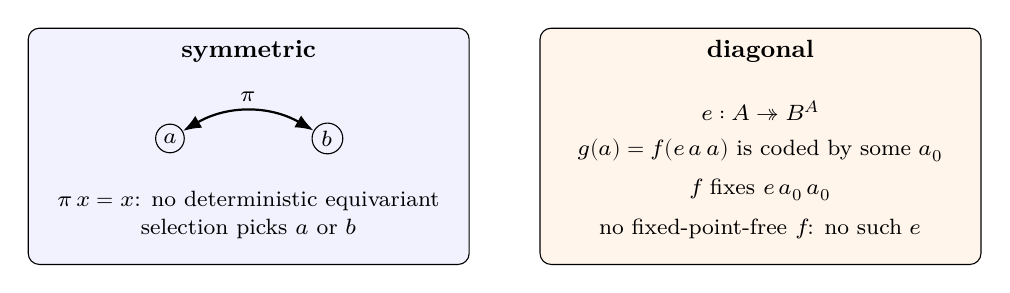
\begin{tikzpicture}[>=Latex, every node/.style={font=\footnotesize},
  box/.style={draw, rounded corners=4pt, minimum width=56mm, minimum height=30mm, align=center}]
  \node[box, fill=blue!5] (sym) at (0,0) {};
  \node[font=\small\bfseries] at (0,1.2) {symmetric};
  \node[circle, draw, inner sep=1.5pt] (a) at (-1,0.1) {$a$};
  \node[circle, draw, inner sep=1.5pt] (b) at (1,0.1) {$b$};
  \draw[<->, thick] (a) to[bend left=30] node[above]{$\pi$} (b);
  \node at (0,-0.7) {$\pi\,x=x$: no deterministic equivariant};
  \node at (0,-1.05) {selection picks $a$ or $b$};
  \node[box, fill=orange!8] (dia) at (6.5,0) {};
  \node[font=\small\bfseries] at (6.5,1.2) {diagonal};
  \node at (6.5,0.45) {$e:A\twoheadrightarrow B^{A}$};
  \node at (6.5,-0.05) {$g(a)=f(e\,a\,a)$ is coded by some $a_0$};
  \node at (6.5,-0.55) {$f$ fixes $e\,a_0\,a_0$};
  \node at (6.5,-1.05) {no fixed-point-free $f$: no such $e$};
\end{tikzpicture}
\caption{Two ineffabilities. Left: at a symmetric state no deterministic equivariant selection
chooses between indiscernibles (Bridge~\ref{thm:symmetry}). Right: a surjection onto its own exponent forces fixed points
(Theorem~\ref{thm:lawvere}).}
\label{fig:twoineffable}
\end{figure}

\subsection{Symmetric ineffability}
\label{sec:symmetric}

A structural description fixes its realizers only up to automorphism. Lewis called the resulting
ignorance \emph{Ramseyan humility}: the Ramsey sentence of a complete physical theory is realized by
any permutation of the fundamental properties that respects its structure, so we cannot know which
property plays which role \cite{Lewis2009}. Bridge~\ref{thm:symmetry} is the formal core. At a state
fixed by a symmetry, no deterministic selection that commutes with the symmetry can pick a member of
an exchanged pair (\code{no\_equivariant\_selection}, \step{ObserverChoices}); and no ultrafilter on $\N$
survives the evens/odds swap (\code{no\_permutation\_invariant\_ultrafilter}), so no free One is chosen
symmetrically.

The scope of the theorem is exact. It excludes a \emph{deterministic} selection that is equivariant
for the stated action, with no choice fixed in advance. It does not exclude other ways of choosing:
an asymmetry or extra state in the record can select, and a uniformly random choice can be
equivariant as a distribution while each of its outcomes breaks the symmetry. The development models
one such alternative. A selection may be a nondeterministic firing whose effect contract includes
recording its choice: taking $5$ and taking $6$ from the sighted pair $\{5,6\}$, each recorded, are
trace equivalent, with records related by the exchange (\code{choice\_recorded\_identified},
\step{ObserverChoices}). That a choice is recorded is part of this firing's contract, not a consequence
of \code{no\_equivariant\_selection}. Where a disclosure is recorded, it shrinks the symmetry group: the
automorphisms of an extended record are those of the record that also fix the extension
(\code{record\_automorphisms\_append}, \step{Fold}).

\paragraph{Local and global.} A related gap concerns the order of quantifiers. Over a set of
solutions of some knowledge, \emph{pointwise} equivalence asks for a matching renaming at each
solution; \emph{uniform} equivalence asks for one renaming that matches at all of them
(\code{pointwiseEquivalent\_iff\_stalks}, \code{moduloEquivalent\_iff\_global},
\step{ObserverSections}). A principal answer is an initial solution, and there the two coincide
(\code{global\_of\_principal}); without one they come apart: two incomparable solutions each have a
matching renaming, and no renaming matches at both (\code{local\_sections\_do\_not\_glue}). This is a
local-versus-global gap in the order of quantifiers, ``for each solution there is a renaming'' against
``there is a renaming for every solution''. It is not contextuality in the sense of overlapping
measurement contexts whose restrictions agree and fail to glue \cite{AbramskyBrandenburger2011}: the
two renamings in the example are not compatible even on the empty overlap. The same split separates
``true in every free One'' from ``true in this One'' in Bridge~\ref{thm:cofinite}.

\begin{reading}[choice among indiscernibles as free choice]
\label{read:freechoice}
One may read Bridge~\ref{thm:symmetry} as saying that no deterministic law can make a choice among
indiscernibles at a symmetric state. A random draw can be symmetric in distribution, while each of its
outcomes breaks the symmetry; recording the outcome is a further contract, not part of the theorem.
Conway and Kochen's free will theorem has a similar shape---a response that is not a function of
the information available to the responder \cite{ConwayKochen2006}---but it is a parallel, not a
consequence: nothing here derives it, and the present theorems concern selections and records, not
physics.
\end{reading}

\begin{remark}[an interpretive aside]
\label{rem:ra}
In the channelled \emph{Law of One} material, free will is named the \emph{first distortion} of the
Law of One \cite{RaMaterial}. Read against the theorem above, the image is apt: no deterministic law
selects at the undivided state, and each outcome of a selection breaks its symmetry. We note
the parallel as interpretation only and draw nothing from it.
\end{remark}

\subsection{Diagonal ineffability}
\label{sec:diagonal}

The second kind is Lawvere's. Theorem~\ref{thm:lawvere} is one statement whose instances are the
classical limits of description: Cantor's theorem that no set maps onto its powerset
\cite{Cantor1891} (\code{cantor\_surjective}), Tarski's undefinability of truth \cite{Tarski1936}
(\code{no\_truth\_predicate}), Curry's paradox read on types (\code{nonempty\_of\_surjective}), the
impossibility of a transparent self-reflection (\code{transparent\_reflection\_impossible},
Theorem~\ref{thm:opaque}), and the collapse of self-containing types
(Theorem~\ref{thm:rationaltypes}). G\"odel's incompleteness theorem \cite{Godel1931} and Chaitin's
bound on the bits of $\Om$ a theory can determine \cite{Chaitin1975} share the diagonal form
\cite{Yanofsky2003}; they are cited here, not formalized.

The two kinds differ in what would remove them. Symmetric ineffability is removed by something
beyond a deterministic equivariant law: a choice fixed in advance, an asymmetry or extra state, or a
random draw whose outcome breaks the symmetry. Diagonal ineffability is removed by no choice at all:
it is a bound on any total internal description, however chosen. The first is a shortage of
structure, the second an excess of reach.

%% ===================================================================
\section{Transforms over transfinite entities}
\label{sec:transforms}

The thesis is about wholes; computation is about steps. This section shows that steps over infinite
wholes behave as the thesis predicts: their limits are characterized by the whole, their conserved
quantities survive passage to the hyperfinite, their silent loops close up to renaming, and a single
cycle can grow without bound.

\paragraph{The candidate step, as far as needed.} A state of the candidate step is a \emph{space}---a
finite set of occurrences, each carrying a labelled term---together with \emph{knowledge}, an equation
store over terms.
A rule's \emph{patterns} say what a firing may do, in five positions: it \emph{takes} occurrences
(consuming them), \emph{reads} occurrences (without consuming them), \emph{makes} new occurrences,
\emph{tells} equations to the knowledge, and is admitted only if its \emph{guards} hold at every
solution of the knowledge. A run is a word of admitted firings. The search combinators
(\code{first}, \code{take}, \code{all}, \code{within}, \step{SearchPolicy}) explore runs under a
budget, with the outcomes of Theorem~\ref{thm:search}. Over rational trees the first-order layer of
the same step runs unchanged; only the meanings of ``solvable'', ``asked'' and ``absent'' change
(Section~\ref{sec:nf-finite}).

\subsection{\texorpdfstring{D1: $\omega$-limits of transforms of infinite trees}{D1: omega-limits of transforms of infinite trees}}
\label{sec:limits}

Let $\mathrm{AgreeBelow}(d,s,t)$ say that two trees have the same label at every path shorter than $d$:
a finite observation. A run of trees \emph{converges} to $t$ when at every depth it is eventually equal
to $t$ below that depth. A transform $\Phi$ of whole trees is \emph{productive} when inputs agreeing
below $d$ give outputs agreeing below $d+1$.

\begin{theorem}[$\omega$-limits; \code{ConvergesTo.unique}, \code{Productive.existsUnique\_fixed},
\code{productive\_guard}, \code{tellLoop\_unfolding\_limit}, \step{TransfiniteLimits}]
\label{thm:limits}
\leavevmode
\begin{enumerate}
\item Limits are unique.
\item A productive transform has exactly one fixed point, and from every start its run of iterates
  converges to it.
\item A guard makes a transform productive: $t\mapsto h(t,\dots,t)$.
\item \emph{The rational step on $X=f(X)$}: the single firing that tells $X=f(X)$ ends in knowledge
  solved by $X:=f(f(f(\cdots)))$; the unfolding run $X,\,f(X),\,f(f(X)),\dots$ converges path-wise to
  that tree; and it is the only tree solving the equation.
\item \emph{Controls}: the transform that flips the root between two constants is not productive and
  none of its runs converges (\code{not\_convergesTo\_rootFlip}, \code{not\_productive\_rootFlip}); the
  unguarded equation $X=X$ has more than one solution (\code{unguarded\_not\_unique}).
\end{enumerate}
\end{theorem}

Part~2 is the contraction principle for the depth ultrametric on trees \cite{ArnoldNivat1980}, read path
by path. Each iterate of the unfolding run is a finite tree, but the limit is not assembled from them:
it is \emph{characterized} as the unique fixed point of a transform of whole trees, and the iterates
are its observations below growing depths. That is Principle~\ref{prin:wholes} in operational form.

\subsection{D2: hyperfinite runs}
\label{sec:hyperrun}

A \emph{conserved charge} of a step is a value on states together with what each firing takes and
makes, balanced at every admitted firing; summed along a run, the books balance (\code{run\_balance},
\step{Charge}), and a run that does not take what it makes cannot fold back to its start
(\code{not\_fold\_of\_unbalanced}). Occurrence weights give such a charge for every step
(\code{weightCharge}). A \emph{hyperfinite run} is a family of runs, one at each index, read modulo an
ultrafilter $\Uf$: its length, its potentials at start and end, and what it takes and makes are germs
along $\Uf$.

\begin{bridge}[charges through an ultrapower; \code{HyperRun.balance}, \code{HyperRun.balance\_weight},
\code{germ\_ne\_iff}, \code{HyperRun.eventually\_not\_fold}, \code{HyperRun.taken\_eq\_made\_of\_eventually\_fold},
\code{HyperRun.const\_lt\_length}, \code{cofinite\_germ\_ne\_not\_eventually\_ne}, \step{TransfiniteUltrapower}]
\label{thm:hyperrun}
\leavevmode
\begin{enumerate}
\item \emph{Conservation}: for every conserved charge, the end potential plus everything taken equals
  the start potential plus everything made, in the ultrapower; in particular for the occurrence
  weights of every step.
\item \emph{The fold filter transfers}: for a charge invariant under the transport, with values in a
  left-cancellative monoid, if the hyperfinite run does not take what it makes, then
  $\Uf$-almost every coordinate run fails to fold back to its start; conversely, if $\Uf$-almost every
  coordinate folds, the hyperfinite run takes what it makes. The proof uses that $\Uf$ is an
  ultrafilter: an inequality of germs is an inequality at $\Uf$-almost every index ({\L}o\'s for a
  negated equation).
\item \emph{Infinite length}: if $\Uf$ is free and, for every $n$, only finitely many coordinate runs
  have length at most $n$, then the length exceeds every standard number.
\item \emph{Control}: over the cofinite filter, which is not an ultrafilter, germs can differ without
  differing eventually (the indicator of the evens against $0$). A reduced power does not suffice;
  the ultrafilter is needed.
\end{enumerate}
\end{bridge}

This is labelled a bridge because a hyperfinite run is assembled from finite coordinate runs, in the
manner of Nelson's radically elementary probability \cite{Nelson1987}. A germ has no coordinates of
its own; what can be read from it is what holds on a set in $\Uf$.

\subsection{Autopoiesis as the quiet fold}
\label{sec:quiet}

A search folds a descendant onto an ancestor when the two lie in one state class. When the observer's
record is carried in the state (the escape-relative transport), folding is restrictive.

\begin{theorem}[the quiet fold; \code{escape\_fold\_quiet}, \code{escape\_fold\_iterates\_quiet}, \step{Fold}]
\label{thm:quiet}
In the escape-relative transport, a run that ends in the class of its start recorded nothing, and
every isomorphism closing it renames by an automorphism of the start's record. Every replay of such a
loop records nothing.
\end{theorem}

\begin{reading}[autopoiesis]
\label{read:autopoiesis}
Maturana and Varela defined an autopoietic system as one whose organization is invariant while its
components are continually replaced \cite{MaturanaVarela1980}. Theorem~\ref{thm:quiet} has that
shape: the organization returns (the state class of the start), while the parts may be renamed (the
closing isomorphism may move occurrence identities), and the renaming is invisible to the environment
(an automorphism of what was disclosed). A loop that discloses cannot close this way: disclosure
shrinks the folding group (\code{record\_automorphisms\_append}). We read self-maintenance as the quiet
fold; the theorem itself concerns runs, records and renamings.
\end{reading}

\subsection{Unbounded growth from one cycle}
\label{sec:pump}

\begin{theorem}[the affine pump; \code{affine\_pump}, \step{FoldPump}]
\label{thm:pump}
Suppose a word of firings $w$ runs from a configuration $C$ and ends in $C\otimes\delta$ up to
equivalence, where every firing of $w$ is query-free (equation guards only, no predicate query),
$\delta$ carries no knowledge, $\delta$ lies beside $C$, and for every finite set of identities there
is a label-keeping renaming that maps the occurrences of $C$ onto themselves and moves what $w$ makes
off that set. Then for every $n$ there
is an executable word ending in $C\otimes E$, where $E$ carries no knowledge, lies beside $C$, and has
$n$ times the labels of $\delta$. \emph{Controls} (\code{producer\_pumps}, \code{absent\_guard\_stops}): a
producer from the empty configuration pumps to $n$ occurrences for every $n$; a rule that makes $b$
while requiring $b$ absent fires once and is then refused, under every renaming.
\end{theorem}

A positive balance alone does not give unbounded growth: the refused control makes one occurrence and
takes none, yet fires only once. Every accumulated frame must keep the cycle admissible, and the
hypotheses say exactly that. Absence and count guards break it, because they are
not blind to what the cycle has already made.

\subsection{The irony, kept explicit}
\label{sec:irony}

Every presentation in this section is finite: a rule with finitely many patterns, a finite graph, a
finite word of firings, a Lean file of a few hundred lines. What these presentations present need not
be finite: an infinite tree characterized as a fixed point, a run whose hyperfinite length exceeds
every number, an unbounded family of configurations from one cycle, an uncountable group of
automorphisms of one whole. This is the first essay's use-versus-mention reply, now with the
mechanisms named. A finite presentation is an observation scheme; it denotes a whole by saying how
the whole may be observed.

%% ===================================================================
\section{Effing the ineffable's boundary}
\label{sec:boundary}

The second half of this essay has a shape that is easy to miss. Its two ineffabilities are not
gestures toward the unsayable; they are \emph{theorems}, finite and checked, and some of them use no
axioms at all. \code{lawvere\_fixedPoint} depends on nothing; \code{select\_ne\_of\_fixed} depends on
nothing; \code{no\_truth\_predicate} and the sinkless collapse use no choice. Each says precisely
where a class of finite presentations must stop: no deterministic equivariant selector at a symmetric
state, no
surjection onto an exponent with a fixed-point-free endomap, no collection of an unfinished search,
no refutation without a finished certificate, no nontrivial model of a self-containing type. The
boundary of effing is itself effed.

This is not a paradox, and it is not the ladder that is thrown away \cite{Wittgenstein1922}. Priest
showed how the diagonal limits of thought share one schema \cite{Priest1995}; Lawvere had already
shown that the classical diagonal arguments are instances of a single fixed-point theorem
\cite{Lawvere1969, Yanofsky2003}. Here the same holds for the symmetric limit: one short form,
\code{select\_ne\_of\_fixed}, carries both the ultrafilter obstruction and the observer obstruction.
The ultrainfinitist position thereby gains a stable shape. The infinite whole is primary (Principle~\ref{prin:wholes}); finite observation reaches it by
prefixes, budgets, coordinates and clopens; and the two places where observation cannot reach are
marked by finite theorems. We do not say the ineffable. We say, exactly, where saying ends.

What remains is foundational work, listed in the next section: the leafless wholes as a final
coalgebra, the Stone points of $\Pfin$, and a genuine ultrapower of the step.

%% ===================================================================
\section{Honest scope}
\label{sec:scope}

\begin{table}[H]
\centering\small
\begin{tabular}{@{}L{0.25\textwidth}L{0.69\textwidth}@{}}
\toprule
Status & Items \\
\midrule
\textbf{Proved} (named anchors) &
  sinkless collapse (Thm.~\ref{thm:sinkless}); leafless plurality (Thm.~\ref{thm:leafless}); inner
  diversity (Thm.~\ref{thm:inner}); no locale points (Thm.~\ref{thm:pointless}); finite shadows,
  continuity as finite-prefix dependence, and finite-resolution observers (Thm.~\ref{thm:shadows},
  Section~\ref{sec:shadow}); opaque atoms
  (Thm.~\ref{thm:opaque}); Lawvere for types and rational
  types (Thms.~\ref{thm:lawvere}--\ref{thm:rationaltypes}); bounded-search outcomes
  (Thm.~\ref{thm:search}); $\omega$-limits (Thm.~\ref{thm:limits}); the quiet fold
  (Thm.~\ref{thm:quiet}); the affine pump (Thm.~\ref{thm:pump}). \\
\textbf{Bridges} (proved; built from finite pieces) &
  B1 the cofinite meet and its {\L}o\'s forms (Bridge~\ref{thm:cofinite}); B2 the symmetry
  obstructions in a form shared with the observer theorem (Bridge~\ref{thm:symmetry}); B3 $\Pfin$
  (Bridge~\ref{thm:pfin}); D2 hyperfinite runs (Bridge~\ref{thm:hyperrun}). Free ultrafilters come
  from choice. \\
\textbf{Readings} (interpretation) &
  the Law of Oneish by structure; plurality by carving; connected, not contractible; the pointless
  One; the empty as an outside view; effable and chosen; that's all $=$ finished; ideal scrutability
  versus effing; free choice among indiscernibles and the Conway--Kochen parallel; the aside on the
  \emph{Law of One}; autopoiesis as the quiet fold; the computable as a shadow. \\
\textbf{Literature, not formalized} &
  the strictness of the effability hierarchy above the rational rung; Chaitin's $\Om$; computable
  normal numbers; pointwise definable models; $\mathrm{St}(\Pfin)\cong\Nstar$; ZF without choice and
  free ultrafilters; G\"odel's theorem; a general Stone space is the inverse limit of its finite
  clopen partitions; computable maps on infinite objects are continuous, in the uniform oracle
  form. \\
\textbf{Open} &
  A3: leafless trees as a final coalgebra, so the core objects are characterized by a universal
  property; the inverse-limit presentation of a general Stone space by its finite shadows, and the
  uniform oracle form of ``computable implies continuous'' (Section~\ref{sec:shadow}); the Stone points of $\Pfin$ are exactly the free ultrafilters on $\N$; admission in an
  ultrapower of the step iff admission at $\Uf$-almost every coordinate, which needs a genuine
  ultrapower of the first-order step; full perfectness, that every leafless tree has a distinct
  neighbour at every depth (Theorem~\ref{thm:leafless}, part~4, gives only some pair at each depth);
  $\omega$-limits for graph systems beyond $X=f(X)$; the symmetry obstruction for every infinite type;
  the coalgebraic, non-well-founded form of opaque atoms. \\
\bottomrule
\end{tabular}
\caption{What is proved, what is a bridge, what is a reading, what is cited, and what is open.}
\label{tab:scope}
\end{table}

\paragraph{Where finitary scaffolding remains.} Principle~\ref{prin:wholes} holds at the object level
of several results while the metatheory and the presentations stay finitary.

\begin{table}[H]
\centering\small
\begin{tabular}{@{}L{0.17\textwidth}L{0.35\textwidth}L{0.39\textwidth}@{}}
\toprule
Result & ``No finite parts'' at the object level & Finitary scaffolding \\
\midrule
sinkless collapse & no member of $\Om$'s closure is empty; $\Om$ is characterized by a property &
  hypersets are quotients of graphs, which may be finite; the closure is reached by finite chains \\
leafless, inner diversity & no leaves; identity carried as structure &
  paths are finite lists; rational trees are counted through finite codes; equality of permutations
  is Lean's equality, not a homotopical identity \\
Lawvere, rational types & a statement about types &
  the collapse to one element decides equality classically; it is a fact about full function spaces
  (Scott's $D\cong[D\to D]$ is nontrivial) \\
$\omega$-limits & the limit is characterized as the unique fixed point &
  its construction reads finite iterates \\
B1, B3, D2 & --- & bridges, defined by finiteness over coordinates; free ultrafilters by choice \\
opaque atoms & ``empty'' is a property of the view &
  a finitary, well-founded syntactic tier \\
\bottomrule
\end{tabular}
\caption{Where ``no finite parts'' holds, and where the scaffolding is still finite.}
\label{tab:scaffolding}
\end{table}

No claim in this essay is stated beyond what its cited anchor proves. The readings are offered as
readings; the bridges are used as bridges.

%% ===================================================================
\appendix

\section{Formalized statements (Lean 4)}
\label{app:lean}

The statements below are transcribed from the source, with Unicode notation spelled in ASCII:
\texttt{forall}, \texttt{exists}, \texttt{<->}, \texttt{!=}, \texttt{in}, \texttt{<=},
\texttt{\textasciitilde=} for an equivalence of types, \texttt{forall\textasciicircum f} for
``eventually'', \texttt{|=} for satisfaction, \texttt{alpha + sigma} for a sum type,
\texttt{<A, s>} for an anonymous constructor, \texttt{*s} for the $n$-fold sum, and Greek letters by
name. Implicit arguments are sometimes omitted. None of the modules contains a hole marker.

\paragraph{Sinkless collapse} (\meta{UltrainfiniteSinkless}).
\begin{lstlisting}
/-- y is in the transitive closure of x, x itself included. -/
def InClosure (x y : HSet) : Prop := Relation.ReflTransGen (fun a b => b in a) x y

/-- Hereditarily nonempty: every member of the closure, itself included, has a member. -/
def HereditarilyNonempty (x : HSet) : Prop := forall y, InClosure x y -> exists z, z in y

/-- Sinkless collapse: two hereditarily nonempty hypersets are equal. -/
theorem eq_of_hereditarilyNonempty (hx : HereditarilyNonempty x)
    (hy : HereditarilyNonempty y) : x = y

/-- The only hereditarily nonempty hyperset is Omega. -/
theorem hereditarilyNonempty_iff_eq_quineAtom :
    HereditarilyNonempty x <-> x = quineAtom

/-- A graph pictures Omega at a node exactly when no sink is reachable from it. -/
theorem decorate_eq_quineAtom_iff_sinkless {a : alpha} :
    decorate r a = quineAtom <-> forall b, Relation.ReflTransGen r a b -> exists c, r b c

/-- With a sink, plurality appears. -/
theorem sink_plurality :
    (emptyset : HSet) != {emptyset} /\ not (HereditarilyNonempty emptyset) /\
      not (HereditarilyNonempty {emptyset})
\end{lstlisting}

\paragraph{Leafless trees and inner diversity} (\meta{UltrainfiniteLeafless},
\meta{UltrainfiniteInnerDiversity}).
\begin{lstlisting}
/-- A leafless tree: well formed, and every label present has a child. -/
def Leafless (t : Raw sigma) : Prop := WF t /\ forall p h, t p = some h -> 0 < h.arity

theorem Leafless.infinite_support (l : Leafless t) : {p | t p != none}.Infinite
theorem not_leafless_ofTerm (u : Term sigma) : not (Leafless (ofTerm u))

theorem not_countable_setOf_leafless (apart : f != g) (pf : 0 < sigma.functionArity f)
    (pg : 0 < sigma.functionArity g) : not {t : Raw sigma | Leafless t}.Countable

theorem countable_leafless_rational [Countable sigma.functionSymbols] :
    {t : Raw sigma | Leafless t /\ IsRational t}.Countable

theorem exists_ne_agree_below (apart : f != g) (pf : 0 < sigma.functionArity f)
    (pg : 0 < sigma.functionArity g) (d : Nat) :
    exists s t : Raw sigma, Leafless s /\ Leafless t /\ s != t /\
      forall p : List Nat, p.length < d -> s p = t p

theorem existsUnique_leafless_of_subsingleton [Subsingleton sigma.functionSymbols]
    (f : sigma.functionSymbols) (pf : 0 < sigma.functionArity f) :
    exists! t : Raw sigma, Leafless t

/-- One whole, many self-identifications. -/
theorem inner_diversity :
    not (Countable treeAut) /\ (forall p, decorate Child p = quineAtom) /\
      forall pi : HSet ~= HSet, (forall x y, y in x <-> pi y in pi x) ->
        pi quineAtom = quineAtom
\end{lstlisting}

\paragraph{Points and opaque atoms} (\lpath{Mettapedia/SetTheory/CarveOuts/HeytingValued/Gunky.lean},
\lpath{Mettapedia/SetTheory/ColoredOpaqueUniverses.lean}).
\begin{lstlisting}
/-- Every point of a complete Boolean algebra is generated by an atom. -/
theorem exists_atom_of_point (p : Point B) :
    exists a, IsAtom a /\ forall h, p.holds h <-> a <= h

/-- An atomless complete Boolean algebra has no point. -/
theorem isEmpty_point_of_isGunky (hg : IsGunky B) : IsEmpty (Point B)

/-- The double-negation part has no two-valued reading. -/
theorem isEmpty_point_regular_opens [T2Space X]
    (noIsolated : forall x : X, not (IsOpen ({x} : Set X))) :
    IsEmpty (Point (Regular (Opens X)))

/-- Opacity: an atom exposes no members, whatever its payload holds. -/
theorem atom_memberless (sees : V.Sees c d) (payload : WfObject V d) (x : WfObject V c) :
    not (MemberOf x (.atom sees payload))

/-- Reference retains identity: distinct payloads give distinct atoms. -/
theorem atom_injective (sees : V.Sees c d) :
    Function.Injective (WfObject.atom (V := V) (c := c) sees)
\end{lstlisting}

\paragraph{Bridges} (\meta{UltrainfiniteCofinite}, \meta{UltrainfiniteCofiniteLos},
\meta{UltrainfiniteSymmetry}, \meta{UltrainfiniteSymmetryObserver}, \meta{UltrainfiniteSetModFinite}).
\begin{lstlisting}
/-- A free ultrafilter: the principal ultrafilter of no point. -/
def IsFree (U : Ultrafilter I) : Prop := forall i, U != pure i

theorem mem_cofinite_iff_forall_free {s : Set I} :
    s in cofinite <-> forall U : Ultrafilter I, IsFree U -> s in U

theorem forall_free_ultraTrue_iff (P : I -> Prop) :
    (forall U : Ultrafilter I, IsFree U -> UltraTrue U P) <-> {i | not (P i)}.Finite

theorem freeOpen_iff (P : I -> Prop) :
    (exists U V : Ultrafilter I, IsFree U /\ IsFree V /\ UltraTrue U P /\
        not (UltraTrue V P)) <->
      {i | P i}.Infinite /\ {i | not (P i)}.Infinite

theorem forall_free_uprod_iff (phi : Sentence L) :
    (forall U : Ultrafilter I, IsFree U -> (Uprod A U) |= phi) <->
      {i | not (A i |= phi)}.Finite

/-- The shared form (no axioms). -/
theorem select_ne_of_fixed (act : X -> X) (act' : Y -> Y) (select : X -> Y)
    (equivariant : forall x, select (act x) = act' (select x)) (fixed : act x = x)
    (apart : a != b) (exchanges : act' a = b /\ act' b = a) :
    select x != a /\ select x != b

theorem no_permutation_invariant_ultrafilter :
    not (exists U : Ultrafilter Nat, forall pi : Equiv.Perm Nat, U.map pi = U)

theorem map_swap_eq_of_isFree [DecidableEq alpha] {U : Ultrafilter alpha}
    (free : IsFree U) (a b : alpha) : U.map (Equiv.swap a b) = U

theorem no_equivariant_selection_of_shared_eq :
    @no_equivariant_selection_of_shared = @AnnotatedRuns.no_equivariant_selection := rfl

abbrev SetModFinite := Germ (cofinite : Filter Nat) Prop
theorem coe_eq_bot_iff (S : Nat -> Prop) : (S : SetModFinite) = bot <-> {n | S n}.Finite
theorem isGunky_setModFinite : IsGunky SetModFinite
theorem perfectSpace_stoneSpace_setModFinite : PerfectSpace (StoneSpace SetModFinite)
\end{lstlisting}

\paragraph{Lawvere and rational types} (\meta{UltrainfiniteLawvere}, \meta{UltrainfiniteLawvereTypes},
\step{RationalTypeControl}).
\begin{lstlisting}
/-- Lawvere's fixed-point theorem for types (no axioms). -/
theorem lawvere_fixedPoint (e : A -> A -> B) (surjective : Function.Surjective e)
    (f : B -> B) : exists b, f b = b

/-- The self-containing type is a One. -/
theorem unique_of_equiv_arrow {X : Sort u} (e : X ~= (X -> X)) : Nonempty (Unique X)

/-- No internal truth predicate. -/
theorem no_truth_predicate (Tr : X -> Prop) (sub : X -> X -> X) :
    not (forall P : X -> Prop, exists c, forall x, Tr (sub c x) <-> P x)

theorem omega_typable : HasType rarrow [] omega (loop .arrow)
theorem omega_no_normal_form (t : Lam) (reached : Relation.ReflTransGen Lam.Beta omega t) :
    exists u, Lam.Beta t u

/-- An arrow model: a type for each rational type, the arrow read as the function type. -/
structure ArrowModel where
  carrier : RTree ctlSig -> Sort u
  arrow : forall a b, carrier (rarrow a b) ~= (carrier a -> carrier b)

theorem rarrow_curryType (b : RTree ctlSig) : rarrow (curryType b) b = curryType b
theorem ArrowModel.unique_carrier (b : RTree ctlSig) : Nonempty (Unique (M.carrier b))

theorem occurs_check_keeps_models :
    (exists M : FiniteArrowModel, exists a b : M.carrier (.const true), a != b) /\
      forall (M : ArrowModel) (b : RTree ctlSig), Nonempty (Unique (M.carrier b))
\end{lstlisting}

\paragraph{Bounded search} (\step{SearchOutcome}, \step{SearchSpace}).
\begin{lstlisting}
inductive Status where | finished | cutOff
structure Outcome (alpha : Type u) where
  answers : Multiset alpha
  status : Status

theorem verdict_ne_refuted_of_cutOff {o : Outcome alpha} (cut : o.status = .cutOff) :
    o.verdict != .refuted

theorem collect_unique [Nonempty alpha] (c : Outcome alpha -> Outcome (Multiset alpha))
    (monotone : Monotone c)
    (onFinished : forall A : Multiset alpha, c <A, .finished> = pure A) : c = collect

theorem run_mono (x : alpha + sigma) : Monotone fun n => S.run n x

theorem status_run_eq_cutOff_iff (n : Nat) (x : alpha + sigma) :
    (S.run n x).status = .cutOff <->
      exists w t, S.item x w = some (.inr t) /\ n <= w.length

theorem refuted_sound (h : (S.approx n x).verdict = .refuted) :
    forall w a, S.item x w != some (.inl a)
\end{lstlisting}

\paragraph{Transforms} (\step{TransfiniteLimits}, \step{TransfiniteUltrapower}, \step{Fold},
\step{FoldPump}).
\begin{lstlisting}
def AgreeBelow (d : Nat) (s t : Raw sigma) : Prop := forall p : List Nat, p.length < d -> s p = t p
def ConvergesTo (run : Nat -> Raw sigma) (t : Raw sigma) : Prop :=
  forall d, exists N, forall n, N <= n -> AgreeBelow d (run n) t
def Productive (Phi : Raw sigma -> Raw sigma) : Prop :=
  forall d s t, AgreeBelow d s t -> AgreeBelow (d + 1) (Phi s) (Phi t)

theorem Productive.existsUnique_fixed (t0 : Raw sigma) :
    exists! a, Phi a = a /\ forall t : Raw sigma, ConvergesTo (fun n => Phi^[n] t) a

theorem HyperRun.balance :
    R.endPotential U Q + R.taken U Q = R.startPotential U Q + R.made U Q

theorem HyperRun.eventually_not_fold [IsLeftCancelAdd A] {T : Transport P}
    (invariant : Q.Invariant T) (unbalanced : R.taken U Q != R.made U Q) :
    forall^f i in U, not (T.Same (R.start i) (R.run i).last)

theorem HyperRun.const_lt_length (free : (U : Filter I) <= cofinite)
    (unbounded : forall n : Nat, {i | (R.run i).word.length <= n}.Finite) (n : Nat) :
    (n : Germ U Nat) < R.length U

theorem cofinite_germ_ne_not_eventually_ne :
    (evenIndicator : Germ (cofinite : Filter Nat) Nat) != (fun _ => 0) /\
      not (forall^f n in cofinite, evenIndicator n != 0)

theorem escape_fold_quiet {x : Escaped P} (r : D.step.Run x)
    (fold : (T.escaping natural D).Same x r.last) :
    r.last.record = x.record /\
      forall i, (T.toStateIso i.base).rename in Record.automorphisms x.record

theorem affine_pump (free : forall f in w, QueryFree f) (runs : Executable A label C w)
    (ends : SameUpTo A (follow label C w) (tensor C delta))
    (spatial : A.Equivalent delta.equations []) (beside : Disjoint C.present delta.present)
    (supply : forall F : Finset O, exists pi : O ~= O, (forall o, label (pi o) = label o) /\
      C.present.map pi.toEmbedding = C.present /\
      Disjoint (madeBy (w.map (Firing.rename pi))) F) :
    forall n : Nat, exists u E, Executable A label C u /\
      SameUpTo A (follow label C u) (tensor C E) /\ A.Equivalent E.equations [] /\
      Disjoint C.present E.present /\
      E.present.val.map label = n *s delta.present.val.map label
\end{lstlisting}

%% ===================================================================
\begin{thebibliography}{99}

\bibitem{UI1} Mettapedia Working Notes. Ultrainfinitism: the finite as a principal-ultrafilter shadow
of the One. Ultraproducts, {\L}o\'s transfer, and imprecise construction for conjecture, credence,
and concept formation. 2026.

\bibitem{AbramskyBrandenburger2011} S.~Abramsky and A.~Brandenburger. The sheaf-theoretic structure
of non-locality and contextuality. \emph{New Journal of Physics}, 13:113036, 2011.

\bibitem{AczelAFA} P.~Aczel. \emph{Non-Well-Founded Sets}. CSLI Lecture Notes~14, Stanford, 1988.

\bibitem{ArnoldNivat1980} A.~Arnold and M.~Nivat. The metric space of infinite trees: algebraic and
topological properties. \emph{Fundamenta Informaticae}, 3(4):445--476, 1980.

\bibitem{BarwiseMoss1996} J.~Barwise and L.~Moss. \emph{Vicious Circles: On the Mathematics of
Non-Wellfounded Phenomena}. CSLI Lecture Notes~60, Stanford, 1996.

\bibitem{BecherFigueira2002} V.~Becher and S.~Figueira. An example of a computable absolutely normal
number. \emph{Theoretical Computer Science}, 270(1--2):947--958, 2002.

\bibitem{BecherFigueiraPicchi2007} V.~Becher, S.~Figueira, and R.~Picchi. Turing's unpublished
algorithm for normal numbers. \emph{Theoretical Computer Science}, 377(1--3):126--138, 2007.

\bibitem{Borel1909} \'E.~Borel. Les probabilit\'es d\'enombrables et leurs applications
arithm\'etiques. \emph{Rendiconti del Circolo Matematico di Palermo}, 27:247--271, 1909.

\bibitem{Cantor1891} G.~Cantor. \"Uber eine elementare Frage der Mannigfaltigkeitslehre.
\emph{Jahresbericht der Deutschen Mathematiker-Vereinigung}, 1:75--78, 1891.

\bibitem{Chaitin1975} G.~J.~Chaitin. A theory of program size formally identical to information
theory. \emph{Journal of the ACM}, 22(3):329--340, 1975.

\bibitem{Chalmers2012} D.~J.~Chalmers. \emph{Constructing the World}. Oxford University Press, 2012.

\bibitem{ChalmersJackson2001} D.~J.~Chalmers and F.~Jackson. Conceptual analysis and reductive
explanation. \emph{The Philosophical Review}, 110(3):315--360, 2001.

\bibitem{Champernowne1933} D.~G.~Champernowne. The construction of decimals normal in the scale of
ten. \emph{Journal of the London Mathematical Society}, 8(4):254--260, 1933.

\bibitem{ComfortNegrepontis1974} W.~W.~Comfort and S.~Negrepontis. \emph{The Theory of
Ultrafilters}. Grundlehren der mathematischen Wissenschaften~211, Springer, 1974.

\bibitem{ConwayKochen2006} J.~Conway and S.~Kochen. The free will theorem. \emph{Foundations of
Physics}, 36(10):1441--1473, 2006.

\bibitem{RaMaterial} D.~Elkins, C.~Rueckert, and J.~McCarty. \emph{The Ra Material} (\emph{The Law of
One}, Book~I). 1984.

\bibitem{Feferman1965} S.~Feferman. Some applications of the notions of forcing and generic sets.
\emph{Fundamenta Mathematicae}, 56(3):325--345, 1965.

\bibitem{GivantHalmos2009} S.~Givant and P.~Halmos. \emph{Introduction to Boolean Algebras}.
Undergraduate Texts in Mathematics, Springer, 2009.

\bibitem{GoertzelHyperseed} B.~Goertzel. \emph{Hyperseed: a scrutability-style core ontology} and
associated concept entries (incl.\ \emph{Unknowability / Infinity / Infinitesimal}: constructive
nonstandard analysis, and \emph{Process}, \emph{Becoming}, \emph{Distinction}). Working manuscripts,
2026.

\bibitem{Godel1931} K.~G\"odel. \"Uber formal unentscheidbare S\"atze der Principia Mathematica und
verwandter Systeme~I. \emph{Monatshefte f\"ur Mathematik und Physik}, 38:173--198, 1931.

\bibitem{Gold1965} E.~M.~Gold. Limiting recursion. \emph{Journal of Symbolic Logic}, 30(1):28--48,
1965.

\bibitem{HamkinsLinetskyReitz2013} J.~D.~Hamkins, D.~Linetsky, and J.~Reitz. Pointwise definable models
of set theory. \emph{Journal of Symbolic Logic}, 78(1):139--156, 2013.

\bibitem{HofmannStreicher1998} M.~Hofmann and T.~Streicher. The groupoid interpretation of type
theory. In G.~Sambin and J.~Smith, editors, \emph{Twenty-Five Years of Constructive Type Theory},
pages 83--111. Oxford University Press, 1998.

\bibitem{HoTTBook} The Univalent Foundations Program. \emph{Homotopy Type Theory: Univalent
Foundations of Mathematics}. Institute for Advanced Study, 2013.

\bibitem{Johnstone1982} P.~T.~Johnstone. \emph{Stone Spaces}. Cambridge Studies in Advanced
Mathematics~3, Cambridge University Press, 1982.

\bibitem{Johnstone1983} P.~T.~Johnstone. The point of pointless topology. \emph{Bulletin of the
American Mathematical Society (N.S.)}, 8(1):41--53, 1983.

\bibitem{Lawvere1969} F.~W.~Lawvere. Diagonal arguments and cartesian closed categories. In
\emph{Category Theory, Homology Theory and their Applications~II}, Lecture Notes in Mathematics~92,
pages 134--145. Springer, 1969.

\bibitem{Lewis2009} D.~Lewis. Ramseyan humility. In D.~Braddon-Mitchell and R.~Nola, editors,
\emph{Conceptual Analysis and Philosophical Naturalism}, pages 203--222. MIT Press, 2009.

\bibitem{MaturanaVarela1980} H.~R.~Maturana and F.~J.~Varela. \emph{Autopoiesis and Cognition: The
Realization of the Living}. Boston Studies in the Philosophy of Science~42, D.~Reidel, 1980.

\bibitem{Nelson1987} E.~Nelson. \emph{Radically Elementary Probability Theory}. Annals of Mathematics
Studies~117, Princeton University Press, 1987.

\bibitem{Pitts2013} A.~M.~Pitts. \emph{Nominal Sets: Names and Symmetry in Computer Science}.
Cambridge Tracts in Theoretical Computer Science~57, Cambridge University Press, 2013.

\bibitem{Priest1995} G.~Priest. \emph{Beyond the Limits of Thought}. Cambridge University Press,
1995.

\bibitem{Putnam1965} H.~Putnam. Trial and error predicates and the solution to a problem of
Mostowski. \emph{Journal of Symbolic Logic}, 30(1):49--57, 1965.

\bibitem{Rutten2000} J.~J.~M.~M.~Rutten. Universal coalgebra: a theory of systems.
\emph{Theoretical Computer Science}, 249(1):3--80, 2000.

\bibitem{Scott1972} D.~Scott. Continuous lattices. In F.~W.~Lawvere, editor, \emph{Toposes, Algebraic
Geometry and Logic}, Lecture Notes in Mathematics~274, pages 97--136. Springer, 1972.

\bibitem{Shoenfield1959} J.~R.~Shoenfield. On degrees of unsolvability. \emph{Annals of Mathematics},
69(3):644--653, 1959.

\bibitem{Stone1936} M.~H.~Stone. The theory of representations for Boolean algebras.
\emph{Transactions of the American Mathematical Society}, 40(1):37--111, 1936.

\bibitem{Tarski1936} A.~Tarski. Der Wahrheitsbegriff in den formalisierten Sprachen. \emph{Studia
Philosophica}, 1:261--405, 1936.

\bibitem{Turing1936} A.~M.~Turing. On computable numbers, with an application to the
Entscheidungsproblem. \emph{Proceedings of the London Mathematical Society} (2), 42:230--265, 1936.

\bibitem{vanMill1984} J.~van~Mill. An introduction to $\beta\omega$. In K.~Kunen and J.~E.~Vaughan,
editors, \emph{Handbook of Set-Theoretic Topology}, pages 503--567. North-Holland, 1984.

\bibitem{Weihrauch2000} K.~Weihrauch. \emph{Computable Analysis: An Introduction}. Texts in
Theoretical Computer Science, Springer, 2000.

\bibitem{Wittgenstein1922} L.~Wittgenstein. \emph{Tractatus Logico-Philosophicus}. Kegan Paul, 1922.

\bibitem{Yanofsky2003} N.~S.~Yanofsky. A universal approach to self-referential paradoxes,
incompleteness and fixed points. \emph{Bulletin of Symbolic Logic}, 9(3):362--386, 2003.

\end{thebibliography}

\end{document}
